\section{Практична частина}
\subsection{Вимірювання заломлюючого кута призми}
\setlength{\parindent}{4em}
\qquadРозрахунок проводиться за наступною формулою
$$\phi =\pi - \beta + \alpha$$\\
Виміряні кути та розрахунки подані у наступній таблиці

\begin{figure}[ht]

\centering

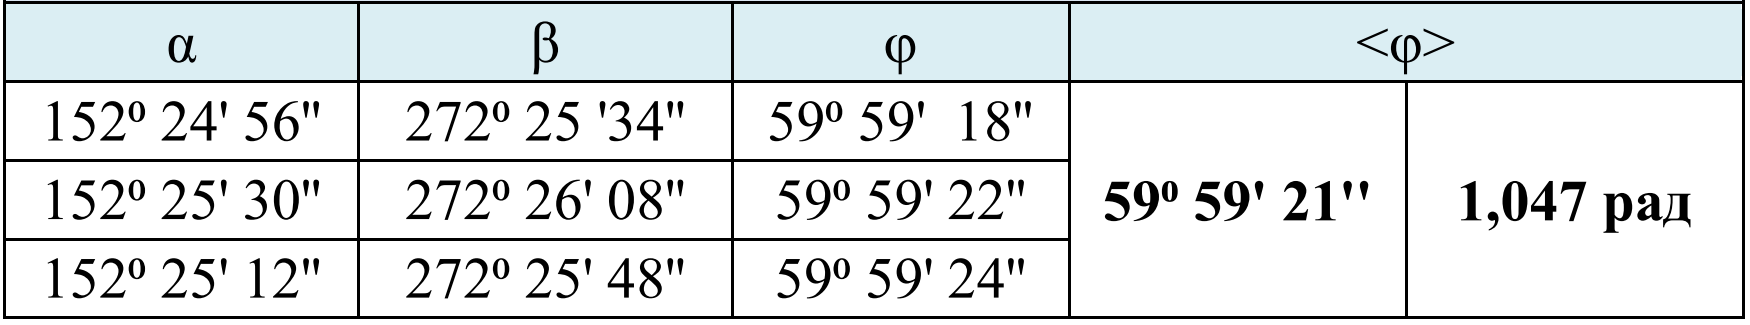
\includegraphics[width=1\linewidth]{Pics/tabl1.png}

\caption{Вимірювання заломлюючого кута призми}

\label{Prac1}

\end{figure}
\subsection{ Визначення кута найменшого відхилення білих ліній спектра ртуті}

\begin{figure}[ht]

\centering

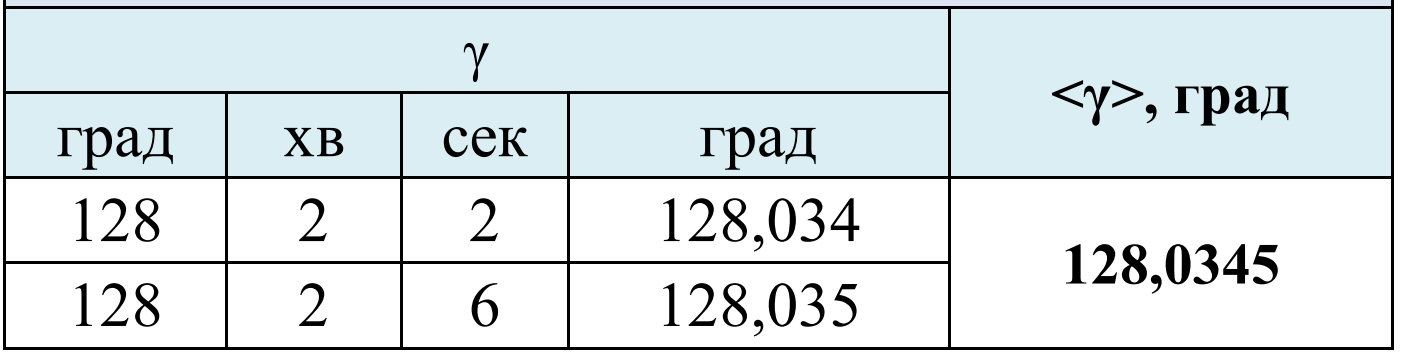
\includegraphics[width=1\linewidth]{Pics/tabl2.png}

\caption{Визначення кута найменшого відхилення}

\label{Prac2}

\end{figure}
\newpage
\subsection{Визначення показників заломлення скла призми для світлових хвиль, що відповідають
різним спектральним лініям ртуті}

\begin{figure}[ht]

\centering

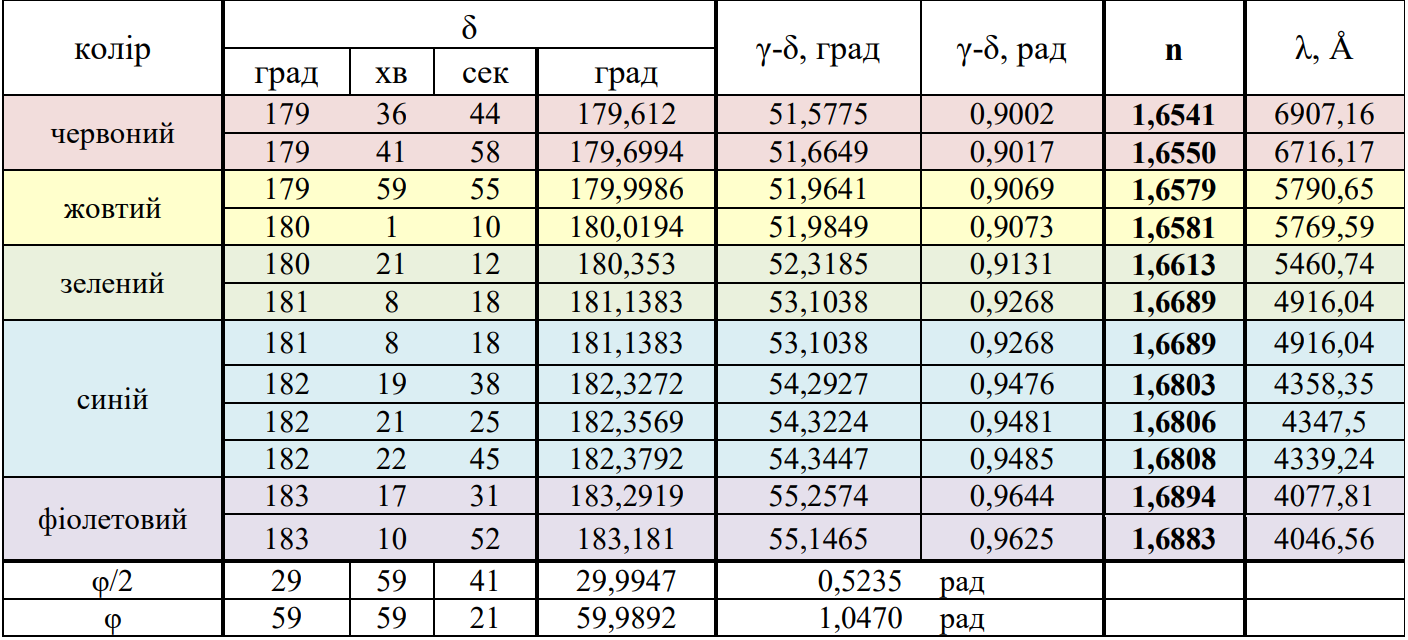
\includegraphics[width=1\linewidth]{Pics/tabl3.png}

\caption{Визначення показників заломлення скла призми}

\label{Prac3}

\end{figure}

\begin{figure}[ht]

\centering

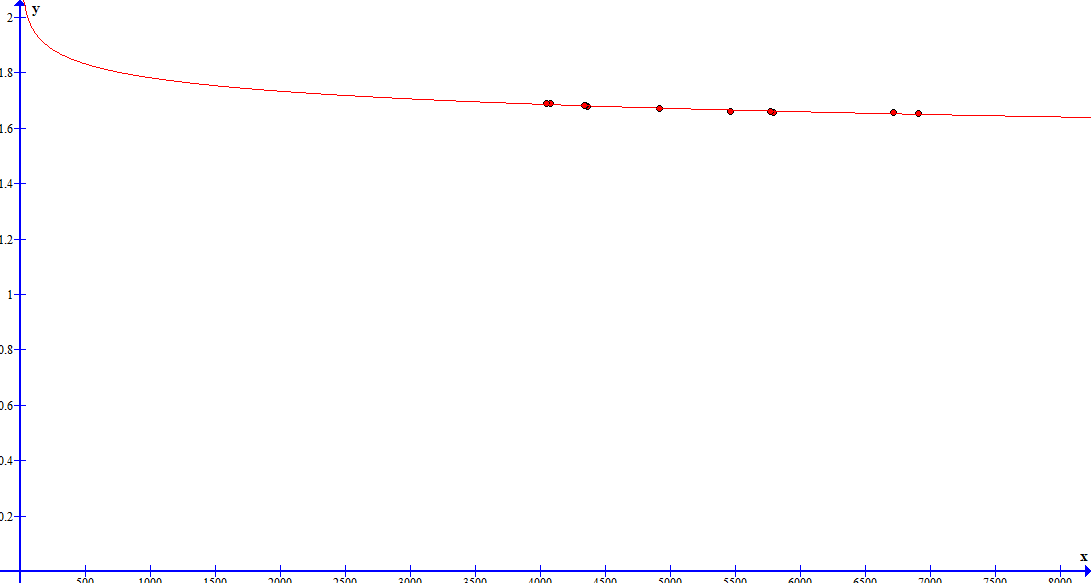
\includegraphics[width=0.9\linewidth]{Pics/tabl5.png}

\caption{Графік залежності показника заломлення від довжини хвилі}

\label{Prac3}

\end{figure}

\newpage
\subsection{Визначення відносної диспервсії скла}
$$N = \frac{n_B + n_R}{n_Y + 1} = \frac{1,6776 + 1,6651}{1,6580+1}$$
